% !Mode:: "TeX:UTF-8"
% !TEX program  = xelatex
\section{Introduction}\label{S:introduction}
\subsection{Preliminary information}
We assume that the reader has already learned the parabola in the physics class and the rectangular coordinate system in the math class. If you do not have the required knowledge, it does not matter, you can follow the information provided in this article, learning while reading.


\subsection{Projectile Motion}
Perhaps we have been told by our parents since childhood that, 45 degrees is the ideal angle to throw a football without air resistance, to understand the reasons why 45 degrees is the best angle without air resistance, we should start with projectile motion\cite{wiki:projectile_motion}.

\begin{defnbox}{Projectile motion}
    Projectile motion is a form of motion experienced by an object or particle (a projectile) that is thrown near the Earth's surface and moves along a curved path under the action of gravity only\footnote{In particular, the effects of air resistance are assumed to be negligible.}.
\end{defnbox}

In the following article, we call the curved path a trajectory\cite{wiki:trajectory}. Through experiments or simulations, we can get the trajectories of football at different angles, as shown in Figure~\ref{F:trajectory}. From the picture we can see that, the footballs are thrown from the origin, the speed remains unchanged, while the angle has changed. Intuitively, 45 degrees is indeed the ideal angle to throw a football for maximum range, and complementary angles have the same range.

The trajectory was shown by Galileo to be a parabola, which is relevant to quadratic equation. No rush, we will learn the basics of quadratic equation, in the next section.

\begin{figure}
    \centering
    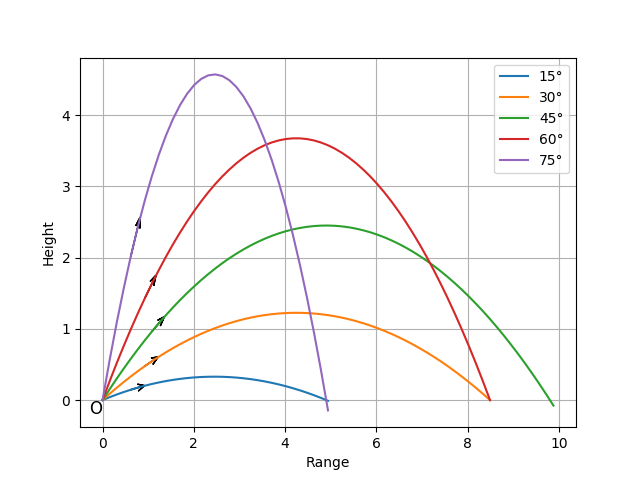
\includegraphics[width=.7\textwidth]{figures/quadratic_equation-1.png}
    \caption{Parabolic trajectories at different angles}\label{F:trajectory}
\end{figure}



\section{Quadratic Equation}\label{S:quadratic}
\subsection{Definition}
\begin{defnbox}{Quadratic equation\cite{wiki:quadratic_equation}}
    In algebra, a quadratic equation (from the Latin \emph{quadratus} for ``square'') is any equation having the form
    \begin{equation}\label{E:1}
        c_2 x^2 + c_1 x + c_0 = 0,
    \end{equation}
    where $x$ represents an unknown, and $c_n$ ($n=0,1,2$) represent known numbers, with $a\neq 0$. If $a=0$, then the equation is linear, not quadratic, as there is no $c_2 x^2$ term. Then we can divide both sides of the equation by $c_2$, and replace $c_1/c_2$ with $b$, $c_0/c_2$ with $c$.
    \begin{equation}\label{E:quadratic-equation}
        x^2 + bx + c = 0.
    \end{equation}
    That is, every quadratic equation can be transformed into the form of Equation~\eqref{E:quadratic-equation}.
\end{defnbox}


\subsection{Quadratic Formula and Its Derivation}
From Equation~\eqref{E:quadratic-equation}, we can complete the square to derive a general formula to solve quadratic equations. Then we have noticed that, coefficient of $x^2$ is 1, coefficient of $x$ is $b$, if we want to complete the square form, we have
\begin{equation}\label{E:quadratic-formula-1}
    \begin{aligned}
        x^2 + bx + c &= 0 \\
        x^2 + 2\frac{b}{2}x &= -c \\
        \left(x+\frac{b}{2}\right)^2 &= -c + \frac{b^2}{4} \\
        \left(x+\frac{b}{2}\right)^2 &= \frac{b^2-4c}{4}.
    \end{aligned}
\end{equation}

The left side of the Equation~\eqref{E:quadratic-formula-1} is a squared form, which means that it may have multiple solutions. That is, if $b^2-4c\geq 0$,
\begin{equation}\label{E:quadratic-formula-2}
    \begin{aligned}
        x + \frac{b}{2} &= \pm \frac{\sqrt{b^2-4c}}{2} \\
        x &= -\frac{b}{2} \pm \frac{\sqrt{b^2-4c}}{2} \\
        x &= \frac{-b\pm\sqrt{b^2-4c}}{2}.
    \end{aligned}
\end{equation}

If we substitute the Equation~\eqref{E:quadratic-formula-2} back to the Equation~\eqref{E:quadratic-equation}, we will find that the equation still holds. That is the quadratic formula is
\begin{equation}\label{E:quadratic-formula}
    x = \begin{cases}
        \frac{-b\pm\sqrt{b^2-4c}}{2} & \text{If $b^2-4c\geq 0$;} \\
        \frac{-b\pm i\sqrt{4c-b^2}}{2} & \text{If $b^2-4c<0$.}
    \end{cases}
\end{equation}

You can get an intuitive feel for the quadratic equation from Figure~\ref{F:quadratic-formula}. Moreover, we found other interesting phenomena --- vertex, which is the extreme point of the parabola, whether minimum or maximum. The $x$-coordinate of the vertex will be located at $x=-\tfrac{b}{2}$, and the $y$-coordinate of the vertex may be found by substituting this $x$-value into the function, which gives that $y=\tfrac{1-(b^2-4c)}{4}$.

\begin{figure}
    \centering
    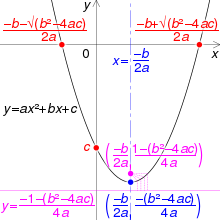
\includegraphics[width=.35\textwidth]{figures/quadratic_equation-2.png}
    \caption{Visualization of quadratic equations (with $a=1$)}\label{F:quadratic-formula}
\end{figure}
